
\begin{figure*}[h!]%
 \centering
 \subfloat[Teirbox indices, from center]{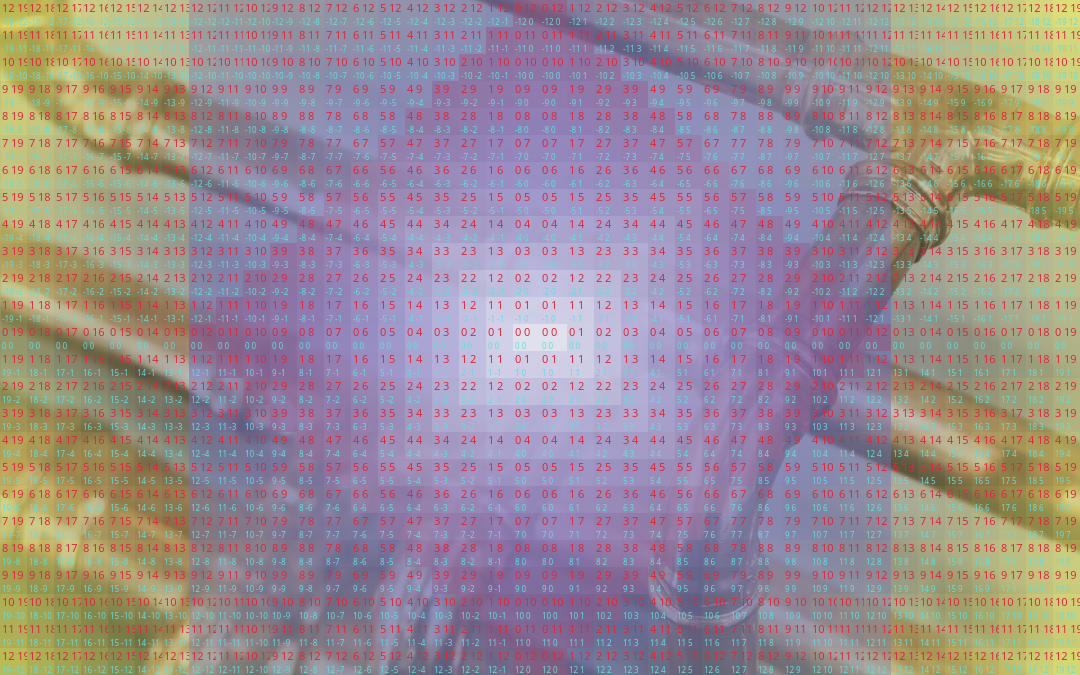
\includegraphics[width=0.6\textwidth]{angle/sh3.png}\label{fig:a}}\\
 \subfloat[Classifying tierboxes by foreground boundary inclusion]{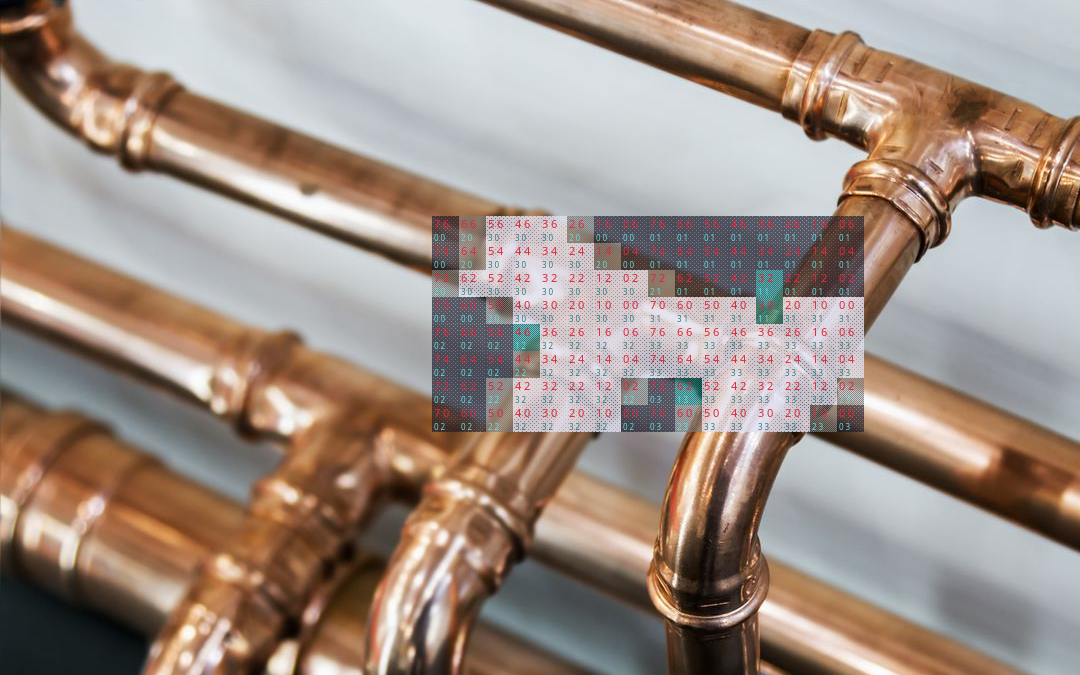
\includegraphics[width=0.5\textwidth, trim=10cm 4.3cm 4.2cm 2.5cm, clip]{angle/sh5.png}\label{fig:a}}\hspace*{1em}%
 \subfloat[Metrics obtained from black-gray lattice constructions]{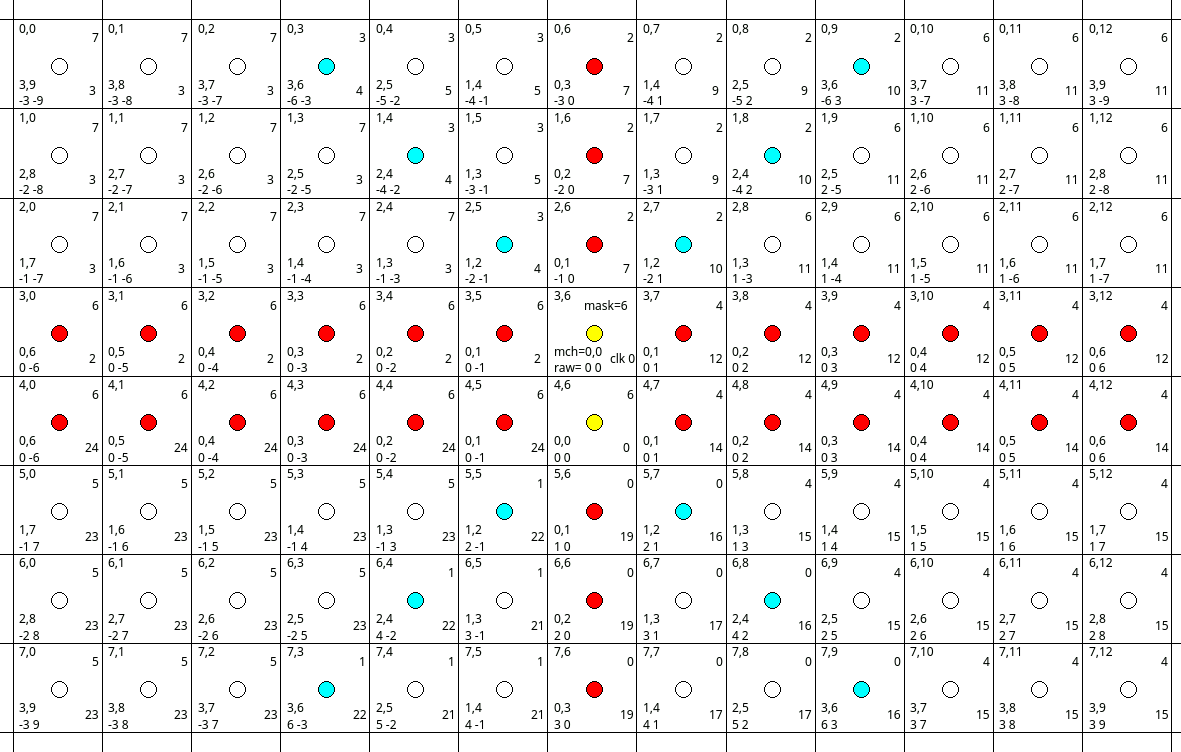
\includegraphics[width=0.5\textwidth, trim=3cm 4mm 3cm 4mm, clip]{angle/sh1b.png}\label{fig:a}}\\
 \subfloat[Gridlines]{\raisebox{2pt}{
\includegraphics[width=\textwidth/2]{angle/grid.png}}\label{fig:c}}\hspace*{1em}%
 \subfloat[Visualizing internal tierbox data]{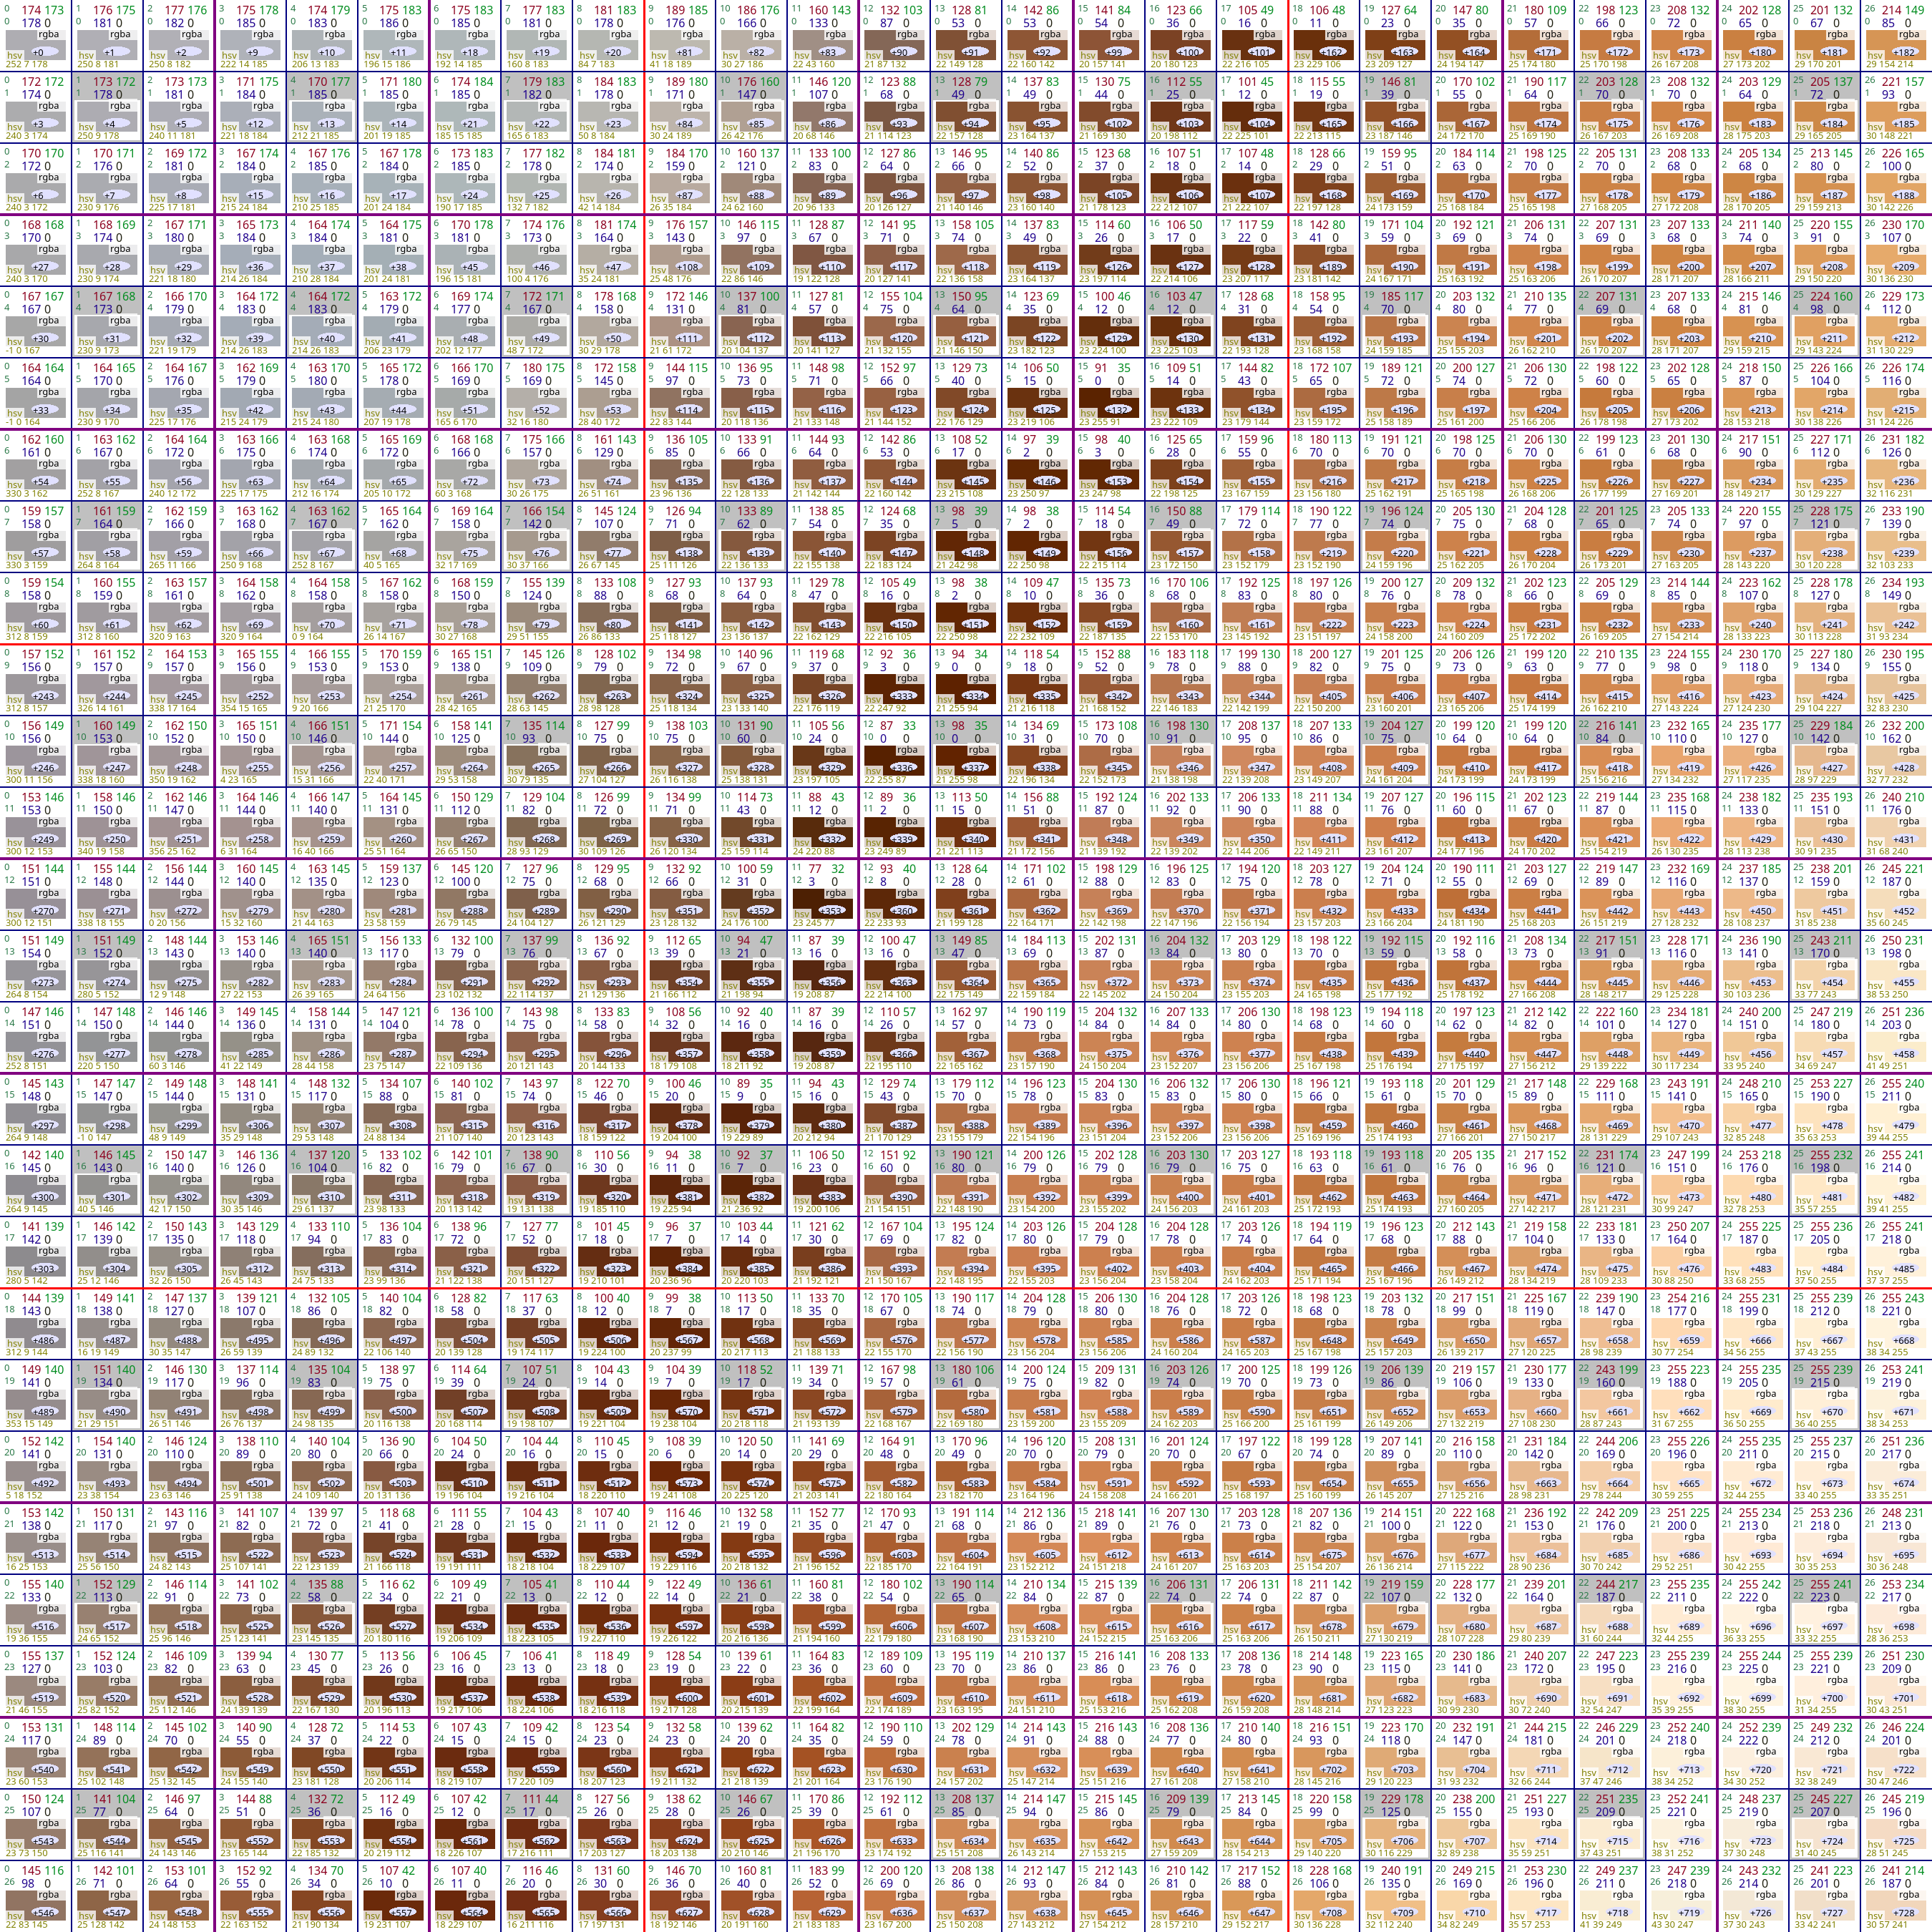
\includegraphics[width=0.51\textwidth, trim=22cm 20cm 34cm 41cm, clip]{angle/sh6.png}\label{fig:d}}\\
 \caption{Visualizing components and quantities for the XCSD format}%
 \label{fig:xcsd-all}%
{\labelbox{XCSD includes various tools for visualizing 
how images are stored internallly according to the 
XCSD protocol, including [a] seeing tierbox indices (data is 
stored from the center outward); [b] foreground and 
region-of-interest boundaries can be defined 
at the tierbox-level; [c] reviewing internal metrics 
XCSD employs to locate pixel memory addresses (according 
to subdivision-indexing);
[d] viewing subdivision-lines into 
(by default 27$\times$27) boxes; [e] generating detailed 
high-zoom summaries of images showing data for 
each pixel and each of the subdivision-scales.}}
\end{figure*}


